\documentclass[11pt,a4paper]{report}

\usepackage[T1]{fontenc}
\usepackage[utf8]{inputenc}
\usepackage[margin=2.5cm]{geometry}
\usepackage{xcolor}
\usepackage{graphicx}
\usepackage{listings}
\usepackage{booktabs}
\usepackage{longtable}
\usepackage{array}
\usepackage{hyperref}
\usepackage{tikz}
\usetikzlibrary{arrows.meta,positioning,shapes.geometric,shapes.multipart,fit,backgrounds,calc}
\usepackage{fancyhdr}
\usepackage{titlesec}
\usepackage{caption}
\usepackage{amsmath}
\usepackage{amssymb}
\usepackage{enumitem}
\usepackage{tcolorbox}
\tcbuselibrary{skins,breakable}
\usepackage{multirow}
\usepackage{pdflscape}

\definecolor{codebg}{RGB}{245,245,245}
\definecolor{fact}{RGB}{0,90,140}
\definecolor{interp}{RGB}{150,90,0}
\definecolor{rec}{RGB}{0,120,60}
\definecolor{warnred}{RGB}{170,30,30}

\lstset{
  basicstyle=\ttfamily\scriptsize,
  backgroundcolor=\color{codebg},
  breaklines=true,
  frame=single,
  numbers=left,
  numberstyle=\tiny\color{gray},
  language=Python,
  keywordstyle=\color{blue!70!black},
  commentstyle=\color{green!40!black},
  stringstyle=\color{purple!60!black}
}

\newtcolorbox{factbox}{colback=fact!5,colframe=fact,fonttitle=\bfseries,title=Observed Fact,breakable}
\newtcolorbox{interpbox}{colback=interp!5,colframe=interp,fonttitle=\bfseries,title=Interpretation,breakable}
\newtcolorbox{recbox}{colback=rec!5,colframe=rec,fonttitle=\bfseries,title=Recommendation,breakable}

\pagestyle{fancy}
\fancyhf{}
\rhead{FDS Visualizer -- Technical Analysis}
\lhead{\leftmark}
\rfoot{\thepage}

\title{
  \vspace{-2cm}
  {\Large Forschungszentrum J\"ulich}\\[0.3cm]
  \rule{\linewidth}{0.5pt}\\[0.4cm]
  {\huge\bfseries Technical Analysis and Research Roadmap\\[0.3cm]
  for the FDS Slice-File Visualizer (\texttt{fds\_visualizer})}\\[0.4cm]
  \rule{\linewidth}{0.5pt}\\[0.5cm]
  {\large A Code Audit, Scientific Visualization Assessment,\\
  and Improvement Plan for a Fire Dynamics Simulator Front-End}
}
\author{Prepared by: Samia Lachgar \\ \small samia.lachgar@um6p.ma}
\date{July 5, 2026}

\begin{document}

\maketitle
\thispagestyle{empty}

\begin{abstract}
\noindent
This report is a full technical audit of the \texttt{fds\_visualizer} repository, a small desktop application
that plays back Fire Dynamics Simulator (FDS) slice-file (\texttt{.sf}) temperature fields as a looping,
kiosk-style animation. The application was built as a public-outreach demonstrator (``Tag der Neugier'')
rather than a research visualization tool, and this shows throughout its design: a single hard-coded
scenario grid, a fixed 1920$\times$1100 full-screen layout, and no configuration, testing, or packaging
infrastructure. The codebase is small (approximately 1{,}070 lines of Python across four files plus one
Qt Designer form) but contains a genuinely reusable and reasonably well-engineered FDS binary-format
parser (\texttt{src/fds/slice/slice.py}) buried underneath a much weaker GUI and data-loading layer. The
report documents the architecture, traces data flow end-to-end, evaluates rendering and performance
characteristics, and separates every claim into \emph{Observed Fact}, \emph{Interpretation}, and
\emph{Recommendation} categories. It concludes with a four-tier roadmap (Quick Wins, Medium, Major,
Research-Level) intended as the starting point for an internship focused on visualization quality,
rendering, responsiveness, data processing, and software architecture.
\end{abstract}

\tableofcontents
\listoffigures
\listoftables

%=====================================================================
\chapter{Executive Summary}
%=====================================================================

\section{What this project actually is}

\begin{factbox}
The repository at \verb|~/Desktop/fds_visualizer| contains exactly 6 Python files.
Excluding the FDS simulation-generation script (\texttt{fds/generate\_sim.py}, out of scope per the
brief) and the empty \texttt{\_\_init\_\_.py}, the application logic totals:
\begin{itemize}[nosep]
  \item \texttt{src/main.py} --- 277 lines --- Qt GUI, event wiring, playback thread.
  \item \texttt{src/load\_data.py} --- 39 lines --- eager bulk loader for all 24 simulation cases.
  \item \texttt{src/fds/slice/slice.py} --- 687 lines --- FDS \texttt{.smv}/\texttt{.sf} binary parser and slice-mesh mapper.
  \item \texttt{src/main\_window.ui} --- a Qt Designer XML form with absolute-pixel widget geometry.
\end{itemize}
There is no \texttt{requirements.txt}, \texttt{pyproject.toml}, \texttt{setup.py}, \texttt{README},
license file, test directory, CI configuration, or logging configuration file anywhere in the
repository. The directory is also not a Git repository (\texttt{git log} run inside it fails --
"not a git repository").
\end{factbox}

\begin{interpbox}
This is a small, single-purpose exhibit application, not a general-purpose visualization tool.
The header comment in \texttt{main.py} (``FDS SLCF Visualizer, FZ-J\"ulich, Max Boehler, Lukas
Arnold, Version 1.0, 2019/06/28'') and the file \texttt{protocol/2019\_05\_21.tex}, which documents a
$2\times3\times3\times2=36$-combination experiment design for a public-outreach event
(``Tag der Neugier'' -- German for ``Day of Curiosity''), confirm that the software was built to
run unattended on a kiosk screen at a science-outreach event, looping a candle/door/vent scenario
matrix. It was never intended as a maintained, extensible research tool, which explains the complete
absence of packaging, testing, and configuration infrastructure. Everything in this report should be
read with that origin in mind: the code is not badly engineered relative to its one-off, one-screen,
one-event purpose -- but it is far from what is needed to serve as the base of a research
internship on visualization quality, rendering, and architecture, which is precisely why the
internship exists.
\end{interpbox}

\section{Key findings at a glance}

\begin{table}[h]
\centering
\begin{tabular}{p{4.2cm}p{9.3cm}}
\toprule
\textbf{Dimension} & \textbf{Verdict} \\
\midrule
Core FDS parser & Reasonably solid binary-format reverse-engineering of FDS \texttt{.sf}/\texttt{.smv} files;
the most reusable asset in the repository. Weak on error handling and API design. \\
Data loading & Eager, blocking, full-precision load of \emph{all} 24 scenarios into a dense
\texttt{float64} 4D array before the GUI opens. No caching, chunking, or lazy loading. \\
Rendering & \texttt{matplotlib} \texttt{imshow} redrawn via \texttt{FigureCanvas.draw()} on every
frame -- a full-figure CPU redraw, not a GPU path, not a blit-based update. \\
Concurrency & A single \texttt{QThread} driven by \texttt{time.sleep} pushes frames via a Qt signal;
stopped with \texttt{QThread.terminate()}, which is unsafe and deprecated practice in Qt. \\
GUI & Fixed full-screen 1920$\times$1100 layout with pixel-absolute widget placement; not
resizable, not scalable to other displays, no keyboard/accessibility support. \\
Scientific visualization & Single 2D scalar heat map, single quantity (temperature), single fixed
slice, gist\_heat colormap (not perceptually uniform), no vector fields, no 3D, no multi-view. \\
Software engineering & No tests, no CI, no logging framework use, no type hints beyond the FDS
parser, no dependency manifest, no version control in the working copy. \\
\bottomrule
\end{tabular}
\caption{High-level verdict summary.}
\end{table}

%=====================================================================
\chapter{Project Overview}
%=====================================================================

\section{Repository layout}

\begin{factbox}
Directory tree (simulation binary payloads collapsed for readability; \texttt{fds/sim/} contains 24
scenario sub-directories, each holding FDS \texttt{.sf}/\texttt{.s3d}/\texttt{.smv}/\texttt{.out}
output files and Slurm batch logs):
\end{factbox}

\begin{lstlisting}[language=bash,basicstyle=\ttfamily\scriptsize]
fds_visualizer/
|-- banner/                     # print assets for the outreach event (out of scope)
|-- fds/
|   |-- generate_sim.py         # HPC batch-job generator (out of scope, see brief)
|   |-- template.fds            # FDS input deck template
|   |-- template_hvac.fds       # FDS input deck template (HVAC variant)
|   |-- start_job.batch         # Slurm submission script
|   `-- sim/                    # 24 pre-computed FDS simulation output folders
|       `-- c{0,1}_d{0,1}_vod{0,1,2}_voc{0,1}/
|           |-- *.smv           # Smokeview geometry/metadata file
|           |-- *.sf            # slice-file binary time series (parsed by slice.py)
|           |-- *.s3d(.sz)      # 3D smoke/soot data (unused by this app)
|           |-- *_hrr.csv       # heat-release-rate time series (unused by this app)
|           |-- *_cpu.csv       # solver performance log (unused by this app)
|           `-- stdout/stderr/*.batch   # HPC job artifacts
|-- image_video_sim/            # exhibit photos / rendered preview media
|-- protocol/                   # LaTeX meeting note defining the 36-case design matrix
`-- src/
    |-- main.py                 # Qt application entry point + GUI controller + playback thread
    |-- load_data.py            # eager bulk loader over fds/sim/*
    |-- main_window.ui          # Qt Designer form (absolute-geometry layout)
    |-- logo/                   # splash screen / window icon assets
    `-- fds/
        |-- __init__.py         # empty (not a real package init)
        `-- slice/
            `-- slice.py        # FDS .smv/.sf binary format parser + slice-mesh mapping
\end{lstlisting}

\section{Provenance and intended use}

\begin{factbox}
\texttt{main.py} lines 1--6 state: ``FDS SLCF Vizualizer -- FZ-J\"ulich -- Max Boehler, Lukas Arnold
-- Version 1.0 -- Date: 2019/06/28.'' \texttt{protocol/2019\_05\_21.tex} defines a design matrix with
axes \emph{Anzahl der Kerzen} (candle count, 2 levels), \emph{T\"urgeometrie} (door geometry, cited as
3 levels in the protocol text but only 2 levels -- \texttt{0.050}, \texttt{0.150} -- are present in
\texttt{fds/generate\_sim.py}), \emph{\"Offnung Decke am Eingang} (entrance ceiling opening: open/
closed/ventilated, 3 levels) and \emph{\"Offnung Decke \"uber Kerze} (candle ceiling opening: open/
closed, 2 levels). The protocol document's own table states ``Anzahl Simulationen: 36'', while
\texttt{generate\_sim.py} and the actual \texttt{fds/sim/} directory both produce
$2\times2\times3\times2 = 24$ simulations.
\end{factbox}

\begin{interpbox}
The mismatch between the planned 36-case matrix and the executed 24-case matrix indicates the door
geometry axis was reduced from 3 to 2 levels between the 2019-05-21 planning meeting and final
execution, without the protocol document being updated. This is a minor documentation inconsistency,
but it is symptomatic of the project's overall lack of any single source of truth: parameter counts
are hard-coded independently in three places (\texttt{generate\_sim.py}, \texttt{load\_data.py}'s call
\texttt{load\_all\_data(2,2,3,2,...)}, and implicitly in the folder-naming convention
\texttt{c\{c\}\_d\{d\}\_vod\{v\}\_voc\{v\}}), and nothing checks that they agree with each other or
with what is actually on disk.
\end{interpbox}

\begin{recbox}
Any refactor should introduce a single declarative scenario manifest (e.g. a JSON/YAML file listing
the factor levels and the resulting folder names) that both the simulation generator and the
visualizer read, eliminating the three-way hard-coded duplication described above.
\end{recbox}

%=====================================================================
\chapter{Architecture Analysis}
%=====================================================================

\section{Component diagram}

\begin{figure}[h]
\centering
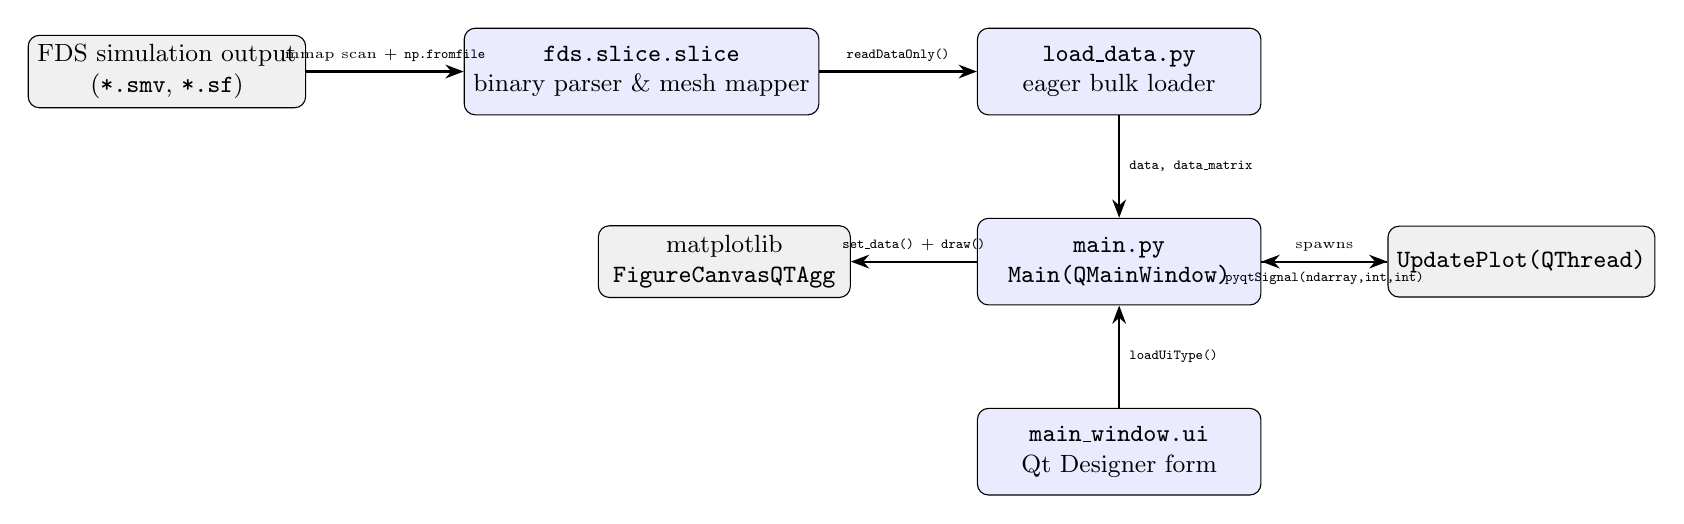
\begin{tikzpicture}[
  box/.style={draw, rounded corners, fill=blue!8, minimum width=3.6cm, minimum height=1.1cm, align=center, font=\small},
  ext/.style={draw, rounded corners, fill=gray!12, minimum width=3.2cm, minimum height=0.9cm, align=center, font=\small},
  arr/.style={-Stealth, thick}
]
\node[ext] (fdsout) {FDS simulation output\\(\texttt{*.smv}, \texttt{*.sf})};
\node[box, right=2.0cm of fdsout] (slice) {\texttt{fds.slice.slice}\\binary parser \& mesh mapper};
\node[box, right=2.0cm of slice] (loader) {\texttt{load\_data.py}\\eager bulk loader};
\node[box, below=1.3cm of loader] (main) {\texttt{main.py}\\\texttt{Main(QMainWindow)}};
\node[ext, right=1.6cm of main] (thread) {\texttt{UpdatePlot(QThread)}};
\node[box, below=1.3cm of main] (ui) {\texttt{main\_window.ui}\\Qt Designer form};
\node[ext, left=1.6cm of main] (mpl) {matplotlib\\\texttt{FigureCanvasQTAgg}};

\draw[arr] (fdsout) -- (slice) node[midway, above, font=\tiny]{mmap scan + \texttt{np.fromfile}};
\draw[arr] (slice) -- (loader) node[midway, above, font=\tiny]{\texttt{readDataOnly()}};
\draw[arr] (loader) -- (main) node[midway, right, font=\tiny]{\texttt{data, data\_matrix}};
\draw[arr] (ui) -- (main) node[midway, right, font=\tiny]{\texttt{loadUiType()}};
\draw[arr] (main) -- (thread) node[midway, above, font=\tiny]{spawns};
\draw[arr] (thread) -- (main) node[midway, below, font=\tiny]{\texttt{pyqtSignal(ndarray,int,int)}};
\draw[arr] (main) -- (mpl) node[midway, above, font=\tiny]{\texttt{set\_data()} + \texttt{draw()}};
\end{tikzpicture}
\caption{Component-level data flow. Everything left of \texttt{load\_data.py} is reusable
FDS-format infrastructure; everything from \texttt{load\_data.py} rightward is exhibit-specific
GUI glue.}
\end{figure}

\section{Import / dependency graph}

\begin{factbox}
Import edges extracted directly from the source files:
\begin{itemize}[nosep]
  \item \texttt{main.py} $\rightarrow$ \texttt{PyQt5} (\texttt{QtCore}, \texttt{QtWidgets}, \texttt{QtGui}, \texttt{uic}), \texttt{numpy}, \texttt{load\_data}, \texttt{matplotlib.figure}, \texttt{matplotlib.backends.backend\_qt5agg}, \texttt{time}, \texttt{sys}.
  \item \texttt{load\_data.py} $\rightarrow$ \texttt{fds.slice.slice} (aliased \texttt{fds}), \texttt{numpy}, \texttt{matplotlib.pyplot} (imported but never used), \texttt{glob}, \texttt{os}.
  \item \texttt{fds/slice/slice.py} $\rightarrow$ \texttt{os}, \texttt{sys}, \texttt{re} (imported, never used), \texttt{tarfile} (imported, never used), \texttt{numpy}, \texttt{matplotlib.pyplot} (imported, never used), \texttt{scipy.interpolate} (imported, never used), \texttt{typing} (imported, only used for a single unenforced return-type hint), \texttt{matplotlib.animation} (imported, never used), \texttt{logging}, and locally \texttt{mmap}, \texttt{glob}, \texttt{os.path}.
  \item \texttt{fds/generate\_sim.py} $\rightarrow$ \texttt{os} only.
\end{itemize}
\end{factbox}

\begin{figure}[h]
\centering
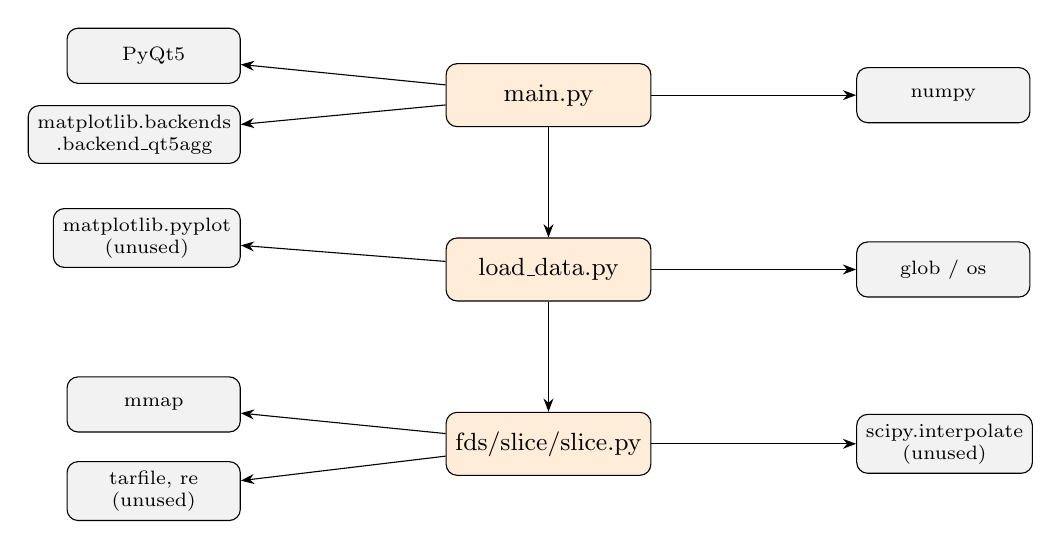
\begin{tikzpicture}[
  node/.style={draw, rounded corners, minimum width=2.6cm, minimum height=0.8cm, align=center, font=\small},
  stdlib/.style={draw, rounded corners, fill=gray!10, minimum width=2.2cm, minimum height=0.7cm, align=center, font=\scriptsize},
  arr/.style={-Stealth}
]
\node[node, fill=orange!15] (main) {main.py};
\node[node, fill=orange!15, below=1.4cm of main] (load) {load\_data.py};
\node[node, fill=orange!15, below=1.4cm of load] (slice) {fds/slice/slice.py};

\node[stdlib, left=2.6cm of main, yshift=0.5cm] (pyqt) {PyQt5};
\node[stdlib, left=2.6cm of main, yshift=-0.5cm] (mplqt) {matplotlib.backends\\.backend\_qt5agg};
\node[stdlib, right=2.6cm of main] (np1) {numpy};

\node[stdlib, right=2.6cm of load] (glob) {glob / os};
\node[stdlib, left=2.6cm of load, yshift=0.4cm] (pltunused) {matplotlib.pyplot\\\scriptsize(unused)};

\node[stdlib, right=2.6cm of slice] (scipyunused) {scipy.interpolate\\\scriptsize(unused)};
\node[stdlib, left=2.6cm of slice, yshift=0.5cm] (mmap) {mmap};
\node[stdlib, left=2.6cm of slice, yshift=-0.6cm] (tar) {tarfile, re\\\scriptsize(unused)};

\draw[arr] (main) -- (pyqt);
\draw[arr] (main) -- (mplqt);
\draw[arr] (main) -- (np1);
\draw[arr] (main) -- (load);
\draw[arr] (load) -- (glob);
\draw[arr] (load) -- (pltunused);
\draw[arr] (load) -- (slice);
\draw[arr] (slice) -- (scipyunused);
\draw[arr] (slice) -- (mmap);
\draw[arr] (slice) -- (tar);
\end{tikzpicture}
\caption{Dependency graph. Orange nodes are project modules; grey nodes are third-party/stdlib
dependencies. Several imports (\texttt{matplotlib.pyplot} in two files, \texttt{scipy.interpolate},
\texttt{tarfile}, \texttt{re}, \texttt{matplotlib.animation}) are dead imports with no call sites
anywhere in the file that imports them.}
\end{figure}

\section{Call graph of the hot path}

\begin{factbox}
Tracing from process start (\texttt{main.py} module-level code, lines 257--277) to the first frame on
screen:
\end{factbox}

\begin{figure}[h]
\centering
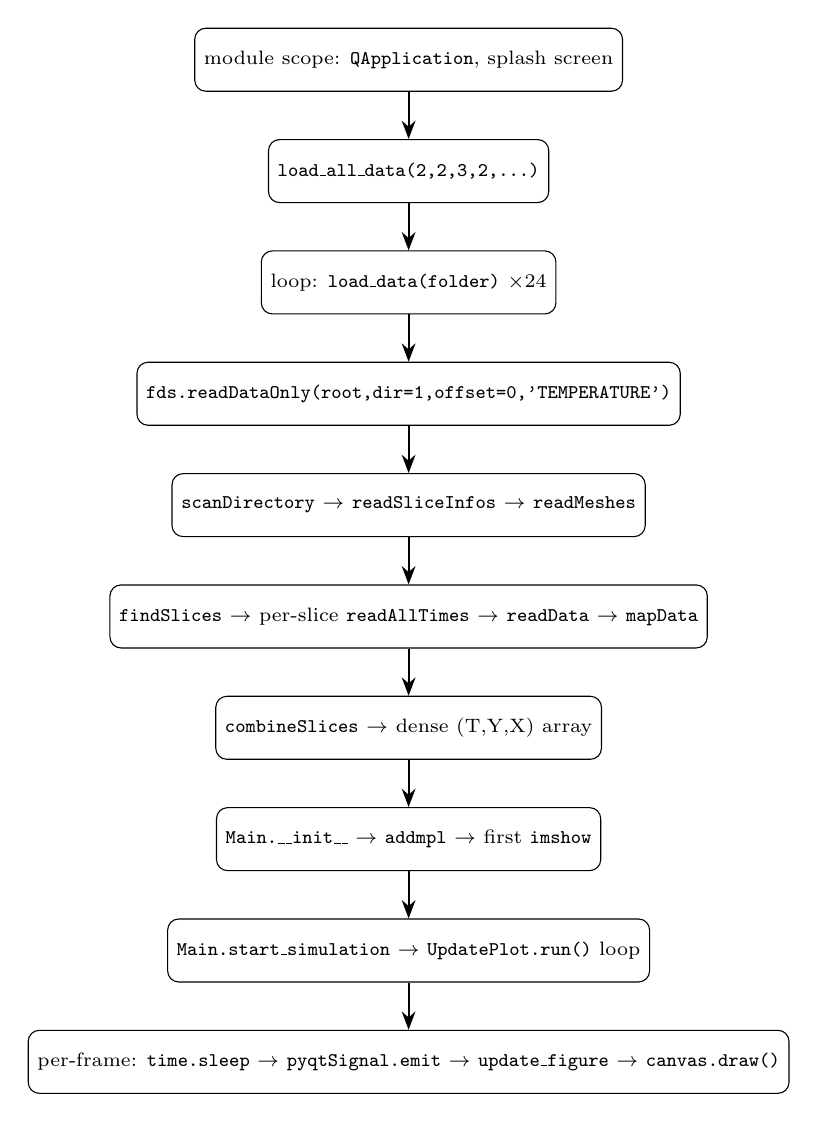
\begin{tikzpicture}[
  n/.style={draw, rounded corners, minimum width=3.4cm, minimum height=0.8cm, align=center, font=\scriptsize},
  arr/.style={-Stealth, thick}
]
\node[n] (a0) {module scope: \texttt{QApplication}, splash screen};
\node[n, below=0.6cm of a0] (a1) {\texttt{load\_all\_data(2,2,3,2,...)}};
\node[n, below=0.6cm of a1] (a2) {loop: \texttt{load\_data(folder)} $\times$24};
\node[n, below=0.6cm of a2] (a3) {\texttt{fds.readDataOnly(root,dir=1,offset=0,'TEMPERATURE')}};
\node[n, below=0.6cm of a3] (a4) {\texttt{scanDirectory} $\to$ \texttt{readSliceInfos} $\to$ \texttt{readMeshes}};
\node[n, below=0.6cm of a4] (a5) {\texttt{findSlices} $\to$ per-slice \texttt{readAllTimes} $\to$ \texttt{readData} $\to$ \texttt{mapData}};
\node[n, below=0.6cm of a5] (a6) {\texttt{combineSlices} $\to$ dense (T,Y,X) array};
\node[n, below=0.6cm of a6] (a7) {\texttt{Main.\_\_init\_\_} $\to$ \texttt{addmpl} $\to$ first \texttt{imshow}};
\node[n, below=0.6cm of a7] (a8) {\texttt{Main.start\_simulation} $\to$ \texttt{UpdatePlot.run()} loop};
\node[n, below=0.6cm of a8] (a9) {per-frame: \texttt{time.sleep} $\to$ \texttt{pyqtSignal.emit} $\to$ \texttt{update\_figure} $\to$ \texttt{canvas.draw()}};

\foreach \i/\j in {a0/a1,a1/a2,a2/a3,a3/a4,a4/a5,a5/a6,a6/a7,a7/a8,a8/a9}
  \draw[arr] (\i) -- (\j);
\end{tikzpicture}
\caption{Call graph of the critical path from process launch to the first steady-state animation
frame. Steps \texttt{a1}--\texttt{a6} (bulk data loading) execute once, synchronously, and block the
Qt event loop except for the single \texttt{app.processEvents()} call inside the loading loop.}
\end{figure}

\section{Sequence diagram: one playback frame}

\begin{figure}[h]
\centering
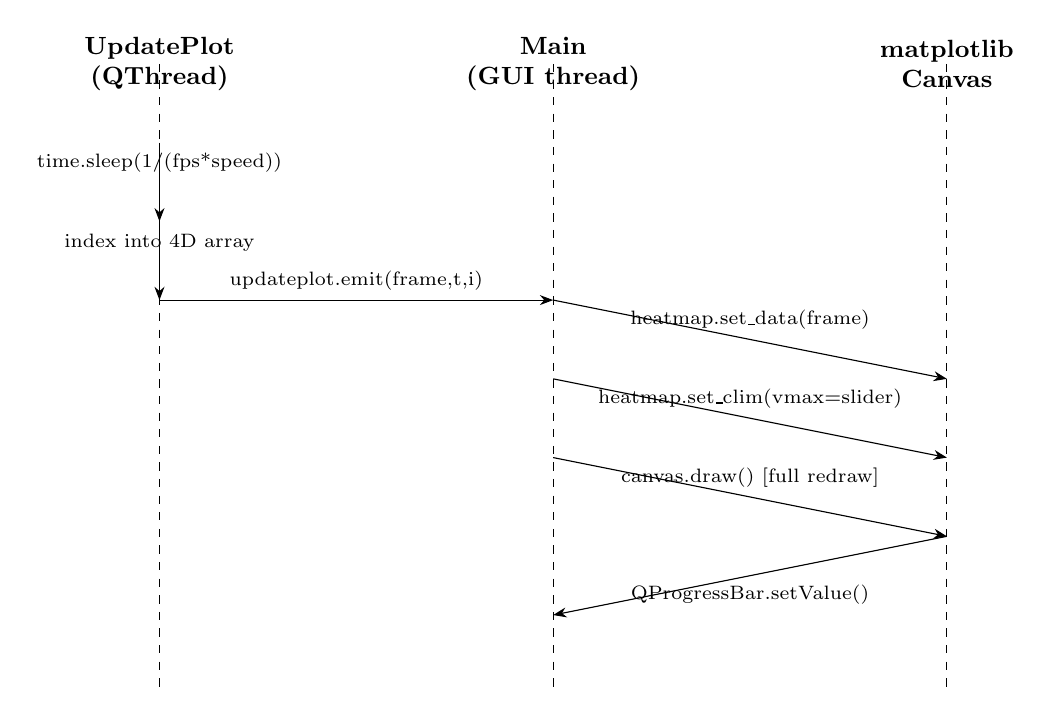
\begin{tikzpicture}[
  actor/.style={font=\small\bfseries, align=center},
  lifeline/.style={dashed},
  msg/.style={-Stealth}
]
\def\yA{6} \def\yB{5} \def\yC{4} \def\yD{3} \def\yE{2} \def\yF{1} \def\yG{0}
\node[actor] (t1) at (0,7) {UpdatePlot\\(QThread)};
\node[actor] (t2) at (5,7) {Main\\(GUI thread)};
\node[actor] (t3) at (10,7) {matplotlib\\Canvas};

\draw[lifeline] (0,7) -- (0,-1);
\draw[lifeline] (5,7) -- (5,-1);
\draw[lifeline] (10,7) -- (10,-1);

\draw[msg] (0,\yA) -- node[above,font=\scriptsize]{time.sleep(1/(fps*speed))} (0,\yB);
\draw[msg] (0,\yB) -- node[above,font=\scriptsize]{index into 4D array} (0,\yC);
\draw[msg] (0,\yC) -- node[above,font=\scriptsize]{updateplot.emit(frame,t,i)} (5,\yC);
\draw[msg] (5,\yC) -- node[above,font=\scriptsize]{heatmap.set\_data(frame)} (10,\yD);
\draw[msg] (5,\yD) -- node[above,font=\scriptsize]{heatmap.set\_clim(vmax=slider)} (10,\yE);
\draw[msg] (5,\yE) -- node[above,font=\scriptsize]{canvas.draw() [full redraw]} (10,\yF);
\draw[msg] (10,\yF) -- node[below,font=\scriptsize]{QProgressBar.setValue()} (5,\yG);
\end{tikzpicture}
\caption{Sequence of one animation tick. The signal crosses from the worker thread to the GUI thread
(Qt handles this marshalling automatically for queued connections), but the actual redraw
(\texttt{canvas.draw()}) is a synchronous, full-figure matplotlib Agg-backend rasterization run
on the GUI thread -- it is not a partial \texttt{blit} update.}
\end{figure}

\section{Class diagram}

\begin{figure}[h]
\centering
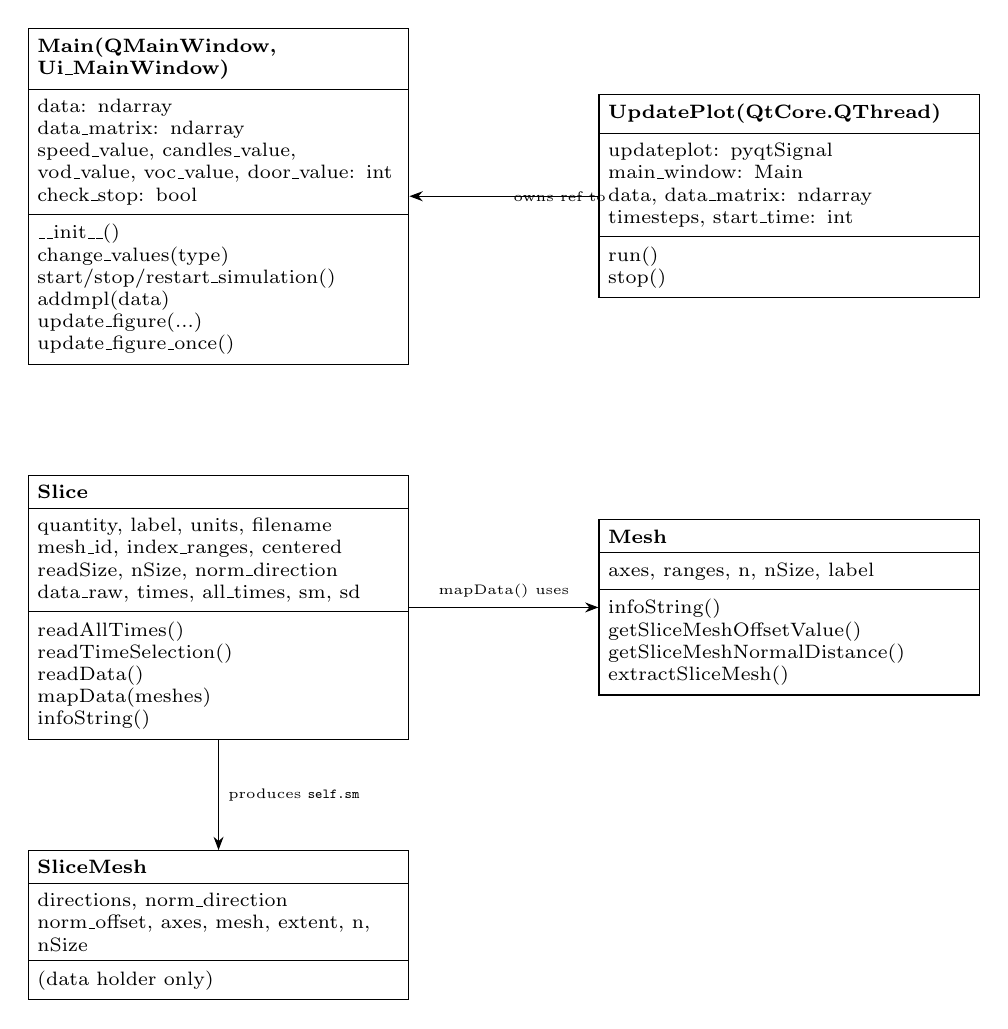
\begin{tikzpicture}[
  cls/.style={draw, rectangle split, rectangle split parts=3, align=left, font=\scriptsize, text width=4.6cm},
  arr/.style={-Stealth}
]
\node[cls] (main) {
  \textbf{Main(QMainWindow, Ui\_MainWindow)}
  \nodepart{second} data: ndarray\\data\_matrix: ndarray\\speed\_value, candles\_value,\\vod\_value, voc\_value, door\_value: int\\check\_stop: bool
  \nodepart{third} \_\_init\_\_() \\ change\_values(type) \\ start/stop/restart\_simulation() \\ addmpl(data) \\ update\_figure(...) \\ update\_figure\_once()
};
\node[cls, right=2.4cm of main] (thread) {
  \textbf{UpdatePlot(QtCore.QThread)}
  \nodepart{second} updateplot: pyqtSignal\\main\_window: Main\\data, data\_matrix: ndarray\\timesteps, start\_time: int
  \nodepart{third} run() \\ stop()
};
\node[cls, below=1.4cm of main] (slice) {
  \textbf{Slice}
  \nodepart{second} quantity, label, units, filename\\mesh\_id, index\_ranges, centered\\readSize, nSize, norm\_direction\\data\_raw, times, all\_times, sm, sd
  \nodepart{third} readAllTimes() \\ readTimeSelection() \\ readData() \\ mapData(meshes) \\ infoString()
};
\node[cls, right=2.4cm of slice] (mesh) {
  \textbf{Mesh}
  \nodepart{second} axes, ranges, n, nSize, label
  \nodepart{third} infoString() \\ getSliceMeshOffsetValue() \\ getSliceMeshNormalDistance() \\ extractSliceMesh()
};
\node[cls, below=1.4cm of slice] (smesh) {
  \textbf{SliceMesh}
  \nodepart{second} directions, norm\_direction\\norm\_offset, axes, mesh, extent, n, nSize
  \nodepart{third} (data holder only)
};
\draw[arr] (thread) -- (main) node[midway,right,font=\tiny]{owns ref to};
\draw[arr] (slice) -- (mesh) node[midway,above,font=\tiny]{mapData() uses};
\draw[arr] (slice) -- (smesh) node[midway,right,font=\tiny]{produces \texttt{self.sm}};
\end{tikzpicture}
\caption{Class diagram. \texttt{MeshCollection} and \texttt{SliceCollection} (simple list wrappers,
omitted for space) complete the parser's data model.}
\end{figure}

\section{Data flow narrative}

\begin{factbox}
\textbf{Where FDS data are loaded:} exclusively in \texttt{src/fds/slice/slice.py}, functions
\texttt{readMeshes} (parses \texttt{GRID}/\texttt{TRNX}/\texttt{TRNY}/\texttt{TRNZ} records from the
\texttt{.smv} text/binary file via a memory-mapped scan), \texttt{readSliceInfos} (parses \texttt{SLC}/
\texttt{SLCC} records for slice metadata), and \texttt{Slice.readData}/\texttt{readAllTimes} (parses
the actual \texttt{.sf} binary time series using \texttt{np.fromfile} with hand-built structured
\texttt{dtype}s that encode Fortran unformatted-record framing, lines 20--42).

\textbf{Where preprocessing occurs:} \texttt{Slice.mapData} (reshapes the flat \texttt{data\_raw}
array into a (time, y, x) grid using the mesh geometry, lines 377--396) and \texttt{combineSlices}
(stitches multiple per-mesh slices into a single global array when a quantity spans more than one
FDS mesh, lines 431--478). \texttt{load\_data.py:load\_data} additionally does \texttt{np.flip(data,
axis=1)} to correct for a vertical-axis convention mismatch between FDS's mesh ordering and
\texttt{imshow}'s default \texttt{origin='upper'} row order.

\textbf{Where rendering occurs:} exclusively in \texttt{src/main.py}, method \texttt{addmpl} (initial
\texttt{Figure}/\texttt{imshow}/\texttt{colorbar} construction, lines 204--218) and
\texttt{update\_figure}/\texttt{update\_figure\_once} (per-frame \texttt{set\_data} + \texttt{set\_clim}
+ \texttt{canvas.draw()}, lines 182--189 and 220--226).

\textbf{Where GUI logic resides:} entirely in \texttt{src/main.py} class \texttt{Main}, which mixes
widget wiring, playback state machine, and rendering calls in one class with no separation of
concerns, plus \texttt{src/main\_window.ui} for static layout.

\textbf{Where visualization algorithms live:} there is exactly one visualization algorithm in the
application -- a 2D pseudocolor raster of a single scalar field via \texttt{matplotlib.imshow}. All
"algorithmic" work (mesh reconstruction, slice combination, coordinate flipping) is data
\emph{preparation}, not visualization per se.

\textbf{Likely performance bottlenecks} (elaborated in Chapter~\ref{ch:perf}): the eager, synchronous,
full-precision load of all 24 scenarios at startup; the per-frame full-figure \texttt{canvas.draw()}
call; and the \texttt{time.sleep}-based frame pacing combined with \texttt{QThread.terminate()} for
stopping playback.
\end{factbox}

%=====================================================================
\chapter{Detailed Code Analysis}
%=====================================================================

\section{\texttt{src/fds/slice/slice.py} (687 lines)}

\subsection{Purpose and responsibilities}
Implements a from-scratch reader for two FDS output formats: the ASCII/binary Smokeview geometry
file (\texttt{.smv}) and the binary slice-file time series (\texttt{.sf}). It reconstructs mesh
coordinate axes, slice metadata, per-timestep scalar fields, and can stitch slices from multiple FDS
meshes into one combined array.

\subsection{Inputs / outputs}
\textbf{Inputs:} a directory path containing one \texttt{.smv} file and one or more \texttt{.sf}
files; a target quantity name (e.g. \texttt{'TEMPERATURE'}), a normal direction (\texttt{0/1/2} or
\texttt{'x'/'y'/'z'}), and an offset index. \textbf{Outputs:} \texttt{readSlice} returns
\texttt{(mesh, extent, data, mask, times)}; \texttt{readDataOnly} (the function actually used by this
application) returns only the dense \texttt{data} array of shape \texttt{(n\_times, n\_y, n\_x)}.

\subsection{Main algorithms}
\begin{itemize}
\item \textbf{Binary layout reconstruction} (\texttt{getSliceType}, lines 20--42): FDS writes
Fortran unformatted sequential files, where each logical record is bracketed by a 4-byte integer
record-length marker (controlled here by the \texttt{fds\_fortran\_backward} flag). The code builds
\texttt{numpy} structured dtypes that read the leading marker, the payload, and the trailing marker in
one \texttt{np.fromfile} call, which is an efficient and idiomatic way to parse Fortran binary output
without a hand-rolled byte-offset parser.
\item \textbf{Memory-mapped text scanning} (\texttt{readMeshes}, \texttt{readSliceInfos}, lines
135--194 and 480--520): uses Python's \texttt{mmap} module with \texttt{bytes.find} to locate
\texttt{GRID}/\texttt{TRNX}/\texttt{TRNY}/\texttt{TRNZ}/\texttt{SLC} tokens inside the \texttt{.smv}
file without loading the whole file into a Python string, then \texttt{seek}+\texttt{readline} to pull
fixed-format numeric fields that follow each token.
\item \textbf{Random-access time-series reads} (\texttt{Slice.readData}, lines 338--373): computes a
fixed \texttt{stride} per timestep record and seeks directly to each timestep's payload, an
$O(n\_times)$ algorithm with $O(1)$ seeks (good practice; avoids a full sequential parse).
\item \textbf{Slice mosaicking} (\texttt{combineSlices}, lines 431--478): computes a bounding box over
all matching slices from potentially different FDS meshes, allocates one dense output array, and
copies each slice's data into its sub-region using pointer arithmetic derived from cell size
\texttt{dx1}/\texttt{dx2}.
\end{itemize}

\subsection{Strengths}
\begin{itemize}[nosep]
\item Uses \texttt{np.fromfile} with structured dtypes rather than manual byte unpacking -- fast and
idiomatic.
\item \texttt{mmap}-based scanning of \texttt{.smv} avoids loading potentially large geometry files
entirely into memory.
\item Correctly separates "reading a slice" (\texttt{readData}) from "mapping onto a mesh"
(\texttt{mapData}) from "combining multiple slices" (\texttt{combineSlices}) -- the closest thing to
good separation of concerns anywhere in the codebase.
\item Domain knowledge is encoded precisely: comments about Fortran record framing and
compiler-dependent binary layout (lines 14--18) show the author understood the fragility of the
format and documented \emph{why}, not just \emph{what}.
\end{itemize}

\subsection{Weaknesses}
\begin{itemize}[nosep]
\item \textbf{No file handles are closed via context managers.} \texttt{readAllTimes},
\texttt{readTimeSelection}, and \texttt{readData} all call \texttt{open(...)} and rely on manual
\texttt{infile.close()} (or, in \texttt{readAllTimes}, never close \texttt{slcf} at all --
line 255--279 opens \texttt{slcf} and it is never closed). On an exception mid-parse, the file
descriptor leaks.
\item \textbf{No error handling anywhere.} Every \texttt{open()}, \texttt{np.fromfile}, and index
lookup assumes well-formed input. \texttt{findSlices} returning an empty list is handled
(\texttt{if len(slices) == 0: print(...); return None}), but a malformed \texttt{.smv} file, a
truncated \texttt{.sf} file, or a mismatched quantity name will raise raw, unhandled exceptions
(\texttt{IndexError}, \texttt{struct} errors) with no context about which file or slice failed.
\item \textbf{Global mutable module state as configuration}: \texttt{fds\_data\_type\_integer},
\texttt{fds\_data\_type\_float}, \texttt{fds\_fortran\_backward} (lines 15--18) are module-level
constants that silently assume a little-endian, 32-bit-int/float, backward-Fortran-record build of
FDS. There is no version detection, no assertion, and no documented way to override them other than
editing the source file.
\item \textbf{Silent correctness assumption in \texttt{norm\_direction}} (\texttt{Slice.\_\_init\_\_},
lines 240--248): if none of the three \texttt{if} conditions match (i.e. the slice is not
axis-aligned on any of the three axes, which should not happen for FDS \texttt{SLC} records but is
never validated), \texttt{self.norm\_direction} is left undefined, and any later access raises an
\texttt{AttributeError} far from the actual root cause.
\item \textbf{Dead/unused imports}: \texttt{re}, \texttt{tarfile}, \texttt{matplotlib.pyplot},
\texttt{scipy.interpolate}, \texttt{matplotlib.animation}, \texttt{typing} (used once, superficially)
are imported but never (or barely) used, inflating apparent dependencies and misleading readers about
what the module actually needs.
\item \textbf{\texttt{readSlice} and \texttt{readDataOnly} are near-duplicates}: lines 539--573 and
575--609 are copy-pasted verbatim except for the final return statement (one returns 5 values, the
other only \texttt{data}). This is a direct SOLID/DRY violation (Section~\ref{sec:solid}).
\item \textbf{Commented-out block of $\sim$80 lines at the end of the file} (lines 611--688) is dead
code left in the module, indicating no cleanup pass was ever done before "shipping."
\item \textbf{No type hints on the vast majority of functions/methods}; a handful of parameters
(\texttt{norm\_dir: str}, \texttt{filename}) have partial hints, but return types, class attributes,
and most parameters are untyped.
\item \textbf{\texttt{readData} always reads every stored timestep, and \texttt{readTimeSelection}
exists but is never called by any code path used in this application} -- meaning the "average over a
time window" and "custom \texttt{dt} resampling" logic is currently unreachable dead functionality
from the app's perspective, even though \texttt{load\_data.py} always wants the same fixed quantity at
full time resolution.
\end{itemize}

\subsection{Complexity, maintainability, scalability}
The parser is $O(T \cdot N)$ per slice for reads ($T$ timesteps, $N$ cells per slice) and
$O(1)$ additional overhead per mesh/slice metadata scan (bounded by \texttt{.smv} file size). This is
close to optimal for the problem. Maintainability is undermined by the duplicated
\texttt{readSlice}/\texttt{readDataOnly} functions and lack of docstrings (only 3 inline explanatory
comments exist in 687 lines). Scalability to larger domains is capped by the fact that
\texttt{Slice.readData} allocates a dense \texttt{np.zeros((n\_times, readSize))} \texttt{float64}
array up front (line 358) -- for a simulation with many timesteps or a large slice this becomes a
large contiguous allocation with no chunking or memory-mapped alternative.

\section{\texttt{src/load\_data.py} (39 lines)}

\subsection{Purpose}
Bulk-loads temperature slice data for every simulation scenario in \texttt{fds/sim/} into one dense
in-memory array and builds an index lookup table (\texttt{data\_matrix}) from the four categorical
scenario factors to a linear scenario index.

\subsection{Main algorithm}
\texttt{load\_all\_data(c, d, vod, voc, progressBar, app)} (lines 12--39):
\begin{enumerate}[nosep]
\item Loads one scenario just to discover the array shape (line 13) -- this means the very first
scenario is parsed from disk \emph{twice}: once to get \texttt{shape}, and again inside the main loop.
\item Counts sub-directories of \texttt{fds/sim/} to size a Qt progress bar (lines 16--19), iterating
the directory listing a second time.
\item Iterates all scenario directories in sorted order, calling \texttt{load\_data} per folder and
writing into a pre-allocated array \texttt{data} of shape
\texttt{(24, n\_time, n\_y, n\_x)} at \texttt{float64} precision (line 14).
\item Builds \texttt{data\_matrix}, a 4D integer array mapping \texttt{(candle, door, vod, voc)}
$\to$ linear index, via a nested loop that simply counts upward (lines 30--36) -- this assumes,
without verifying, that \texttt{sorted(glob.iglob(...))} enumerates folders in exactly the same
lexicographic order as the nested loop's iteration order. Because the folder names are
\texttt{c\{i\}\_d\{j\}\_vod\{k\}\_voc\{l\}}, lexicographic sort of the string \emph{does} coincide with
the nested-loop counting order for single-digit indices -- but this is an unstated invariant, not an
enforced one.
\end{enumerate}

\subsection{Strengths}
Minimal, does what it needs to for a fixed, known dataset; using a Qt \texttt{QProgressBar} plus
\texttt{app.processEvents()} at least keeps the splash screen responsive during the otherwise blocking
load (line 27).

\subsection{Weaknesses}
\begin{itemize}[nosep]
\item \textbf{Hard-coded relative paths}: \texttt{'../fds/sim/c1\_d0\_vod0\_voc0/'} (line 13) and
\texttt{'../fds/sim/**'} (lines 16, 22) assume the process's current working directory is
\texttt{src/} at launch. There is no path resolution relative to the module's own location
(\texttt{os.path.dirname(\_\_file\_\_)}), so running the app from any other working directory silently
fails or loads the wrong data.
\item \textbf{Loads all 24 scenarios eagerly and unconditionally at startup}, at full \texttt{float64}
precision, even though only one scenario is ever displayed at a time and the GUI can switch scenarios
interactively via buttons. For the current dataset ($24 \times 121 \times \sim\!60\times\!40$-ish
grids) this is tolerable, but it is an $O(\text{all scenarios})$ startup cost for an
$O(\text{one scenario})$ steady-state need, and it does not scale if the number of scenarios,
resolution, or timesteps grows.
\item \textbf{Silent broad \texttt{except} in the caller}: \texttt{main.py} wraps the call to
\texttt{load\_all\_data} in a bare \texttt{try/except:} (lines 268--271) that catches
\emph{every} exception type and prints one generic "did you forget git-lfs" message, discarding the
actual traceback. Any real bug in parsing, a missing folder, a permissions error, or an out-of-memory
condition looks identical to the user.
\item \textbf{Unused import}: \texttt{matplotlib.pyplot} (line 3) is never referenced.
\item \textbf{Redundant double-scan of the directory}: the sub-directory count loop (lines 16--18) and
the main load loop (line 22) both call \texttt{glob.iglob('../fds/sim/**')} independently instead of
listing once and reusing the list.
\item \textbf{Duplicate \texttt{progressBar.setValue(i)} calls} (lines 25 and 28) inside the same loop
iteration -- harmless but indicates the loop was edited without cleanup.
\item \textbf{No caching to disk}: every application launch re-parses all 24 scenarios' full binary
slice files from scratch; nothing is memoized (e.g. to a \texttt{.npy}/\texttt{HDF5}/\texttt{Zarr}
cache keyed on file mtimes).
\end{itemize}

\section{\texttt{src/main.py} (277 lines)}

\subsection{Purpose}
Application entry point: builds the \texttt{QApplication}, shows a splash screen while data loads,
constructs the main window, and implements the GUI's event handling and playback control.

\subsection{Class \texttt{Main(QMainWindow, Ui\_MainWindow)}}
\textbf{Responsibilities (too many for one class):} Qt widget initialization; a five-factor scenario
selector state machine (\texttt{speed}, \texttt{candles}, \texttt{vod}, \texttt{voc}, \texttt{door}) implemented via
16 near-identical \texttt{if/elif} branches in \texttt{change\_values} (lines 77--160); animation
lifecycle management (\texttt{start\_simulation}, \texttt{stop\_simulation}, \texttt{restart\_simulation});
and direct matplotlib figure manipulation (\texttt{addmpl}, \texttt{update\_figure},
\texttt{update\_figure\_once}). This is a textbook God Object: one class owns UI wiring, application
state, business logic (which scenario maps to which array slab), \emph{and} rendering.

\subsection{Class \texttt{UpdatePlot(QtCore.QThread)}}
A worker thread whose \texttt{run()} method (lines 239--251) is an infinite \texttt{while True} loop
that sleeps for \texttt{1/(timesteps*speed\_value)} seconds, reads the currently selected scenario's
next frame from the shared \texttt{data} array, and emits it via a Qt signal. Playback is stopped by
calling \texttt{QThread.terminate()} (line 254), which forcibly kills the OS thread at an
arbitrary point -- Qt's own documentation calls this ``a dangerous function'' because it can leave the
thread's resources (in this case, nothing critical, but this is not guaranteed for all future
maintainers) in an undefined state, and it is explicitly discouraged in favor of a cooperative
stop flag.

\subsection{Strengths}
\begin{itemize}[nosep]
\item Uses a background \texttt{QThread} plus a \texttt{pyqtSignal} to update the GUI, correctly
avoiding direct cross-thread widget mutation (Qt widgets are not thread-safe, and this code does not
touch them from the worker thread).
\item The overall flow (splash $\to$ load $\to$ show window $\to$ start on demand) is a sensible
shape for a kiosk application.
\end{itemize}

\subsection{Weaknesses}
\begin{itemize}[nosep]
\item \textbf{\texttt{change\_values} is a 16-branch \texttt{if/elif} chain keyed on a hard-coded
string} (lines 77--160), setting \texttt{.setEnabled()} flags on button pairs/triples by hand. Adding
one more factor level requires copy-pasting and hand-editing at least 3--4 more branches, and there is
no exhaustiveness check -- an unmatched \texttt{type} string silently falls through doing nothing.
\item \textbf{A dangling reference bug}: \texttt{self.speed\_1.setEnabled(False)} etc. at
\texttt{\_\_init\_\_} time (lines 52--56) disable buttons \emph{before} the corresponding
\texttt{clicked} handlers are connected -- functionally fine here, but the ordering is fragile and
undocumented (a reader cannot tell whether this ordering matters without tracing every line).
\item \textbf{Race condition risk between the worker thread and the main thread}: \texttt{UpdatePlot.run()}
reads \texttt{self.main\_window.speed\_value}, \texttt{candles\_value}, \texttt{door\_value},
\texttt{vod\_value}, \texttt{voc\_value} every iteration (line 243) while the GUI thread can mutate
those same attributes at any time via button clicks (\texttt{change\_values}, called from the Qt event
loop). Because these are plain Python \texttt{int} attribute reads/writes (atomic under the GIL) this
does not currently corrupt memory, but it is an unsynchronized shared-mutable-state pattern that is
fragile and would break under any richer state (e.g. a compound object) without warning.
\item \textbf{\texttt{stop\_simulation} vs. \texttt{start\_simulation} leaks threads}: each call to
\texttt{start\_simulation}/\texttt{restart\_simulation} constructs a brand-new \texttt{UpdatePlot}
instance and calls \texttt{.start()} (lines 165--167, 193--198) without first waiting
(\texttt{.wait()}) for a prior thread's \texttt{terminate()} to actually finish. In principle this
allows two \texttt{UpdatePlot} threads to be alive simultaneously, both holding references to
\texttt{self.data}, both emitting signals to the same slot.
\item \textbf{Hard-coded, absolute-pixel, full-screen UI}: \texttt{main\_window.ui} specifies a fixed
$1920\times1100$ window and every widget has an absolute \texttt{<geometry>} rect; \texttt{main.py}
calls \texttt{self.showFullScreen()} unconditionally (line 32) and re-enters full screen on any
double-click (\texttt{mouseDoubleClickEvent}, lines 162--163). On any monitor other than exactly
1920$\times$1080/1100, widgets will be cropped, misaligned, or leave dead space -- there is no layout
manager (\texttt{QVBoxLayout}/\texttt{QGridLayout}) used for the top-level widgets, only for the
matplotlib canvas container (\texttt{mplvl}).
\item \textbf{No way to exit full-screen except the on-screen ``Exit'' button}, and no keyboard
shortcuts (e.g. Esc, F11) are wired -- an accessibility and usability gap.
\item \textbf{\texttt{loadUiType('main\_window.ui')}} (line 26) and the icon/splash paths
(\texttt{'logo/fds\_vis\_small.png'}, line 33; \texttt{'logo/fds\_vis.png'}, line 260) are all relative
paths resolved against the current working directory, not the module's location -- identical fragility
to the one documented in \texttt{load\_data.py}.
\item \textbf{Global/module-level executable code} (lines 257--277) runs at import time with no
\texttt{if \_\_name\_\_ == '\_\_main\_\_':} guard, meaning \texttt{main.py} cannot be imported (e.g.
by a test suite or by another entry point) without immediately launching the full GUI application and
blocking.
\item \textbf{Duplicated code}: \texttt{start\_simulation} and \texttt{restart\_simulation} (lines
165--172, 193--202) are identical except for resetting \texttt{start\_time = 1} first.
\end{itemize}

\subsection{\texttt{src/main\_window.ui}}
A Qt Designer XML form using \texttt{QWidget}s placed at absolute pixel coordinates rather than
Qt layout managers (\texttt{QGridLayout}, \texttt{QFormLayout}), except for the single
\texttt{QVBoxLayout} (\texttt{mplvl}) that hosts the matplotlib canvas. This is consistent with
(and the direct cause of) the fixed-resolution assumption baked into \texttt{main.py}.

%=====================================================================
\chapter{Scientific Visualization Analysis}
%=====================================================================

\section{How the scalar field is visualized}

\begin{factbox}
The application visualizes exactly one scalar field, FDS quantity \texttt{'TEMPERATURE'}
(\texttt{load\_data.py}, line 8), extracted as a single axis-aligned 2D slice
(\texttt{direction=1, offset=0}, i.e. a slice normal to the $y$-axis at mesh index 0). It is rendered
with \texttt{matplotlib.axes.Axes.imshow(data, cmap='gist\_heat')} (\texttt{main.py}, line 207) and a
single shared \texttt{colorbar} (line 211). The colorbar upper limit is interactively adjustable via a
\texttt{QSlider} (\texttt{temp}, range 30--300, mapped to \texttt{heatmap.set\_clim(vmax=...)}),
while the lower limit is left at matplotlib's automatic default from the first frame.
\end{factbox}

\subsection{Mathematical description of the rendering pipeline}
Let $T(x,y,t)$ be the discretized temperature field on the FDS slice mesh, of shape
$(n_y, n_x)$ at each of $n_t$ discrete times. \texttt{imshow} maps each cell $T_{i,j,t}$ to a
color via a piecewise-linear normalization
\[
  n_{i,j,t} = \operatorname{clip}\!\left(\frac{T_{i,j,t} - v_{\min}}{v_{\max} - v_{\min}},\; 0,\; 1\right)
\]
followed by a lookup into the \texttt{gist\_heat} colormap function
$C: [0,1] \to \mathbb{R}^3$ (RGB). Here $v_{\min}$ is fixed at the first frame's data minimum (never
updated), and $v_{\max}$ is the live slider value (\texttt{self.temp.value()}), so
\emph{every subsequent frame is normalized against a stale, frame-0-derived $v_{\min}$}. If later
frames' minimum temperature drifts (physically plausible as the fire evolves and cooling occurs
elsewhere in the domain), the color mapping's lower end silently becomes inaccurate.

\subsection{Slice extraction and combination}
Mathematically, \texttt{Mesh.extractSliceMesh} projects the 3D mesh axes $(x_1,x_2,x_3)$ onto the two
axes orthogonal to \texttt{norm\_dir}, producing a 2D mesh via \texttt{np.meshgrid}. When more than one
FDS sub-mesh contributes to the same physical plane, \texttt{combineSlices} performs a mosaicking
operation: it computes a global bounding box
$[\min x_1, \max x_1] \times [\min x_2, \max x_2]$ over all contributing slices' extents, assumes a
uniform, shared cell size $(dx_1, dx_2)$ taken from the \emph{first} slice only (line 444--445 --
this silently assumes all meshes share identical resolution, which is not verified), and copies each
slice into its computed offset sub-region of one dense array. This is effectively nearest-neighbor
tiling, not true interpolation: no resampling occurs across mesh boundaries, so any two meshes with
different resolution would either misalign or (worse) silently overwrite adjacent data because the
offset arithmetic (\texttt{int((s.sm.extent[0] - min\_x1) / dx1)}) uses truncating integer division.

\subsection{Animation and temporal navigation}
\begin{factbox}
Animation is implemented as literal wall-clock-paced frame stepping: \texttt{UpdatePlot.run()}
sleeps for $1/(f \cdot s)$ seconds per frame, where $f{=}4$ is the fixed \texttt{DT\_SLCF}-derived
frame rate (\texttt{self.timesteps = 4}, \texttt{main.py} line 43, hard-coded to match the FDS input
deck's slice output interval of 0.25s) and $s \in \{1,2,3\}$ is the user-selected speed multiplier.
There is no scrubbing, no seek bar the user can drag, no pause-at-frame, and no reverse playback --
\texttt{time\_progress} (a \texttt{QProgressBar}, not a \texttt{QSlider}) is read-only display, not an
interactive seek control, despite occupying the most prominent horizontal strip of the window.
\end{factbox}

\begin{interpbox}
Because frame pacing is \texttt{time.sleep}-based rather than driven by a Qt \texttt{QTimer} or a
monotonic-clock-corrected scheduler, actual playback speed will drift under system load: each loop
iteration's total period is $\text{sleep duration} + \text{(signal emission, GUI-thread redraw, and
signal round-trip latency)}$, none of which is accounted for. On a loaded system, or if
\texttt{canvas.draw()} takes longer than one frame period (very plausible, see
Chapter~\ref{ch:perf}), frames will visibly stutter or the animation will fall behind real simulation
time without any compensation.
\end{interpbox}

\section{GUI update mechanism and rendering backend}

\begin{factbox}
Rendering uses \texttt{matplotlib}'s \texttt{Qt5Agg} backend (\texttt{FigureCanvasQTAgg}), which
rasterizes the entire matplotlib \texttt{Figure} in software via the Anti-Grain Geometry (Agg) library
on the CPU, then blits the resulting raster image into the Qt widget. There is no
\texttt{pyqtgraph}, no \texttt{VisPy}, no raw \texttt{QOpenGLWidget}, and no GPU-accelerated rendering
path anywhere in the codebase.
\end{factbox}

\begin{interpbox}
\texttt{canvas.draw()} (called every frame in \texttt{update\_figure}, line 223) is matplotlib's
"redraw everything" API -- it re-renders axes, colorbar, and image from scratch on every call, as
opposed to \texttt{canvas.draw\_idle()} combined with \texttt{blit} of only the changed \texttt{Artist}
(the \texttt{AxesImage} returned by \texttt{imshow}). Because the colorbar and axes are static between
frames (only the temperature array and the color-limit change), this is a clear case of a CPU-bound,
non-vectorized-at-the-rendering-level bottleneck: every frame pays for re-rendering static content
that never changes.
\end{interpbox}

%=====================================================================
\chapter{Performance Analysis}
\label{ch:perf}
%=====================================================================

\section{Computational and memory bottlenecks}

\begin{table}[h]
\centering
\small
\begin{tabular}{p{3.3cm}p{4.6cm}p{2.2cm}p{4.0cm}}
\toprule
\textbf{Location} & \textbf{Issue} & \textbf{Complexity} & \textbf{Consequence} \\
\midrule
\texttt{load\_all\_data} & Eager load of all 24 scenarios at \texttt{float64} before GUI opens;
first scenario parsed twice (shape probe + main loop) & $O(S \cdot T \cdot N)$, $S{=}24$ scenarios & Startup latency scales linearly with total scenario count and grid size; blocks event loop except for one \texttt{processEvents()} call \\
\texttt{Slice.readData} & Allocates \texttt{np.zeros((n\_times, readSize))} at \texttt{float64}, one \texttt{np.fromfile} call per timestep (not one bulk read) & $O(T)$ syscalls, $O(T \cdot N)$ memory & $T$ separate seek+read syscalls per slice instead of one strided/bulk read; doubles memory vs. \texttt{float32} source precision \\
\texttt{combineSlices} & Nearest-neighbor tiling with integer-truncated offsets, no interpolation & $O(M \cdot N)$, $M$=meshes & Silent misalignment risk if meshes have unequal cell size (unvalidated assumption) \\
\texttt{update\_figure} & Full \texttt{canvas.draw()} every frame instead of \texttt{blit} & $O(\text{full figure raster})$ per frame & CPU-bound per-frame cost dominated by re-rendering unchanged axes/colorbar chrome \\
\texttt{UpdatePlot.run} & \texttt{time.sleep}-paced infinite loop with no drift compensation & -- & Playback speed is not guaranteed real-time-accurate under load \\
\bottomrule
\end{tabular}
\caption{Identified bottlenecks, their asymptotic behavior, and consequences.}
\end{table}

\section{I/O bottlenecks}
\begin{itemize}[nosep]
\item Every application launch re-reads and re-parses all 24 scenarios' \texttt{.smv} and \texttt{.sf}
files from disk with no caching layer -- for a "look at a fixed exhibit" use case this is repeated,
avoidable I/O on every kiosk reboot.
\item \texttt{Slice.readAllTimes} performs one \texttt{np.fromfile(count=1)} call per timestep in a
Python-level \texttt{while True} loop (lines 264--279) to discover how many timesteps exist, rather
than computing the count directly from file size and the known per-record stride -- an
easily-vectorizable operation left as a scalar Python loop.
\end{itemize}

\section{GUI / concurrency bottlenecks and thread safety}
\begin{itemize}[nosep]
\item \texttt{QThread.terminate()} (main.py line 254) is documented by Qt as unsafe: it can be called
at any point in the thread's execution, including mid-instruction, and provides no opportunity for
cleanup. The correct pattern is a cooperative boolean flag checked each loop iteration plus
\texttt{wait()} after requesting a stop.
\item No mutex/lock protects the scenario-selection integers read by the worker thread and written by
the GUI thread (Section 4.3, \texttt{UpdatePlot.run} vs. \texttt{Main.change\_values}). Currently benign
under CPython's GIL for simple int attributes, but it is an unsynchronized-shared-state anti-pattern.
\item Starting a new \texttt{UpdatePlot} thread without confirming the previous one's
\texttt{terminate()} has completed (no \texttt{.wait()}) creates a window where two threads can be
alive and emitting to the same Qt slot concurrently.
\end{itemize}

\section{NumPy usage assessment}
The FDS parser's use of \texttt{np.fromfile} with structured dtypes is idiomatic and efficient. However,
\texttt{Slice.readData}'s per-timestep loop (\texttt{for t in range(...): infile.seek(...);
np.fromfile(...)}, lines 363--370) is a case where a single strided/bulk read (e.g. reading the whole
file as one structured array with \texttt{count=n\_times} using the known fixed stride, or using
\texttt{np.memmap}) would replace $T$ Python-level iterations and syscalls with one vectorized call.
This is the clearest "non-vectorized operation that should be vectorized" in the codebase.

%=====================================================================
\chapter{GUI Analysis}
%=====================================================================

\section{Layout and navigation}
\begin{factbox}
The interface is a single, non-resizable, full-screen window with no menus, tabs, or navigation of
any kind (the \texttt{QMenuBar} in \texttt{main\_window.ui} is present but empty -- no
\texttt{QAction}s are defined). All 15 interactive widgets (5 scenario-factor button groups, 3 playback
buttons, 1 slider, 1 progress bar) are visible simultaneously on one screen.
\end{factbox}

\section{Usability findings}
\begin{itemize}[nosep]
\item \textbf{No way to know which scenario is currently selected at a glance} beyond which button is
disabled (the "selected" state is encoded as \texttt{setEnabled(False)} on the chosen option, which is
a strong overload of a control that normally means "unavailable," not "currently active" -- a
significant accessibility/legibility issue since a disabled (usually greyed-out) button is easy to
misread as "this option cannot be chosen" rather than "this option is already chosen").
\item \textbf{No numeric readout of simulation time}, only \texttt{time\_progress} showing seconds via
its \texttt{\%v sec.} format string -- functional but minimal.
\item \textbf{No confirmation or visual feedback while data is loading} beyond the initial splash
screen's progress bar; if loading takes long (e.g. on slower storage), the app gives no further
indication that it has not frozen.
\item \textbf{Restart requires stop-then-restart}, and \texttt{simulation\_restart} is only enabled
after \texttt{stop\_simulation} is clicked (line 176) -- there is no direct "restart from beginning
while playing" action.
\item \textbf{No keyboard interaction at all}: no shortcuts, no focus indicators, no way to operate the
application without a mouse/touchscreen, which is a real limitation for an accessibility standard and
even for a public kiosk (some venues require keyboard/switch-access alternatives).
\end{itemize}

\section{Missing features (from a scientific-visualization-tool perspective)}
No zoom/pan, no probe/read-out of the value under the cursor, no ability to change the visualized
quantity or slice plane, no colorbar auto-rescale toggle, no screenshot/export function, no side-by-side
comparison of two scenarios, no legend for what the button rows mean physically beyond static labels.

%=====================================================================
\chapter{Rendering / Graphics Quality Analysis}
%=====================================================================

\section{Current rendering quality}
\begin{factbox}
Colormap: \texttt{gist\_heat}, a non-perceptually-uniform, non-colorblind-safe matplotlib colormap
(it is not one of matplotlib's "perceptually uniform sequential" maps such as \texttt{inferno},
\texttt{magma}, or \texttt{viridis}). Resolution: rendered at native slice-grid resolution with
\texttt{imshow}'s default \texttt{interpolation='antialiased'} (matplotlib $\geq 3.x$ default, i.e.
mild automatic smoothing only, not a deliberate choice in this code). No anti-aliasing options are
explicitly set. No lighting, shading, transparency, or depth cues are used because the visualization is
strictly 2D.
\end{factbox}

\section{Opportunities and why they matter scientifically}
\begin{table}[h]
\centering
\small
\begin{tabular}{p{3.4cm}p{5.4cm}p{5.4cm}}
\toprule
\textbf{Opportunity} & \textbf{Current state} & \textbf{Scientific justification} \\
\midrule
Perceptually uniform colormap (\texttt{inferno}/\texttt{magma}) & \texttt{gist\_heat}, uneven perceptual steps & Equal data differences must map to equal perceived color differences, or viewers misjudge gradient steepness -- critical for interpreting a temperature field's spatial gradient correctly \\
Fixed, non-drifting normalization & $v_{\min}$ frozen at frame 0, $v_{\max}$ user-set & A static, physically-meaningful reference range (e.g. ambient to a fixed hazard threshold) avoids visually misrepresenting later frames \\
Bilinear/bicubic interpolation for display & Native grid resolution, default matplotlib interpolation & Smoother apparent gradients better convey continuous physical fields without implying false grid-cell discreteness \\
Streamlines / vector glyphs & Not present; only scalar temperature is loaded & FDS also outputs velocity slices; visualizing flow direction alongside temperature reveals convective transport that a scalar field alone hides \\
Clipping planes / multi-slice & Single fixed slice at \texttt{offset=0} & A single 2D cut cannot show 3D fire plume structure; multiple parallel slices or an interactive cut plane reveal vertical stratification \\
Volume rendering & Not present & FDS \texttt{.s3d} smoke/soot data exists on disk but is unused by this app; volumetric rendering would convey plume shape directly \\
Side-by-side multi-view & Single view of one scenario at a time & The dataset's entire purpose is comparing 24 scenarios; a linked multi-panel view is the single highest-value visualization feature missing \\
GPU-accelerated rendering & CPU Agg rasterization via matplotlib & Removes the per-frame full-redraw bottleneck and enables higher frame rates / larger grids without stutter \\
\bottomrule
\end{tabular}
\caption{Rendering and visual-quality improvement opportunities, ranked roughly by expected
scientific value per engineering effort.}
\end{table}

%=====================================================================
\chapter{Simulation Visualization Improvements}
%=====================================================================

\begin{itemize}
\item \textbf{Lazy / on-demand loading}: load only the currently selected scenario (and prefetch
adjacent ones) instead of all 24 up front. Rationale: the GUI can display only one scenario at a time
(\texttt{data\_matrix} selects a single index), so eager-loading the other 23 is pure wasted I/O and
memory for every session; this directly shortens perceived startup time.
\item \textbf{Disk-backed caching (e.g. \texttt{.npy}/\texttt{Zarr}/HDF5) keyed on source file
mtimes}: avoids re-parsing binary \texttt{.sf} files on every launch when the underlying simulation
output has not changed.
\item \textbf{Chunked / memory-mapped reads (\texttt{np.memmap}) in \texttt{Slice.readData}}: replaces
the current per-timestep Python loop and dense \texttt{float64} allocation with a lazily-paged view,
reducing both peak memory and load latency, and enabling datasets larger than RAM.
\item \textbf{Progressive/streaming load with immediate first-frame display}: show frame 0 as soon as
it is parsed rather than waiting for the entire time series of the entire scenario matrix.
\item \textbf{Blit-based animation instead of full \texttt{canvas.draw()}}: re-render only the
\texttt{AxesImage} artist per frame; static chrome (axes, colorbar) is drawn once. This is a purely
rendering-side fix requiring no changes to the data model.
\item \textbf{Timer-based (QTimer) frame pacing instead of \texttt{time.sleep} in a QThread}: removes
drift and the need for \texttt{terminate()}-based thread teardown, since a \texttt{QTimer} can simply
be stopped.
\item \textbf{Temporal interpolation between stored timesteps} is not currently needed (source data is
evenly spaced at 0.25s and displayed at native resolution) but would become relevant if variable-rate
playback or synchronization across scenarios of different simulated durations is added.
\end{itemize}

%=====================================================================
\chapter{Software Engineering Review}
%=====================================================================

\section{Architecture and modularity}
\begin{interpbox}
The project has a reasonable \emph{physical} split (parser vs. loader vs. GUI) but a poor
\emph{logical} one: \texttt{Main} in \texttt{main.py} concentrates widget wiring, a five-factor state
machine, playback lifecycle, and direct matplotlib manipulation in a single 200-line class with no
internal decomposition. There is no model/view separation of any kind: the "model" (which scenario is
selected, at what time) and the "view" (matplotlib figure, Qt widgets) are updated by the same methods
with no intermediate abstraction a test or a different front-end could target.
\end{interpbox}

\section{SOLID violations}
\label{sec:solid}
\begin{itemize}[nosep]
\item \textbf{Single Responsibility}: \texttt{Main} handles UI events, application state, and
rendering. \texttt{Slice} handles both binary parsing (\texttt{readData}) and geometric remapping
(\texttt{mapData}) -- workable at this size, but already blurring the line.
\item \textbf{Open/Closed}: adding a new scenario factor (e.g. a 5th binary variable) requires editing
\texttt{change\_values}'s \texttt{if/elif} chain, the \texttt{main\_window.ui} layout, and
\texttt{load\_all\_data}'s hard-coded shape/loop -- nothing is closed to modification.
\item \textbf{DRY (not strictly SOLID but closely related)}: \texttt{readSlice}/\texttt{readDataOnly}
in \texttt{slice.py} and \texttt{start\_simulation}/\texttt{restart\_simulation} in \texttt{main.py}
are near-verbatim duplicates.
\end{itemize}

\section{Testing, CI, configuration, error handling}
\begin{factbox}
No test files, no test framework dependency, no CI configuration (no \texttt{.github/workflows},
no \texttt{.gitlab-ci.yml}), no \texttt{requirements.txt}/\texttt{pyproject.toml}, no
\texttt{logging.getLogger(\_\_name\_\_)}-per-module pattern (only \texttt{slice.py} configures the
root logger once, at \texttt{CRITICAL} level -- effectively disabling all its own \texttt{logging.debug}
calls by default), and exactly one broad, swallowing \texttt{except:} clause in the entire codebase
(\texttt{main.py}, line 270).
\end{factbox}

\begin{recbox}
Priority order for a research internship: (1) pin dependencies in a \texttt{pyproject.toml}; (2)
extract the FDS parser into an installable, independently testable package with unit tests against
known-good \texttt{.sf} fixtures; (3) introduce a thin ViewModel/state layer between \texttt{Main} and
the plotting code so rendering logic becomes testable without a running Qt event loop; (4) replace the
blanket \texttt{except:} with targeted exception handling that preserves the traceback in a log file.
\end{recbox}

%=====================================================================
\chapter{Research Opportunities}
%=====================================================================

\begin{itemize}
\item \textbf{Multi-scenario linked comparison views}: since the dataset's entire scientific purpose is
comparing 24 parametric variations, a synchronized small-multiples or linked-cursor comparison view
(shared time axis, shared color scale) is both a strong visualization-research topic (small-multiples
design for parametric ensembles) and directly useful to the underlying fire-safety experiment.
\item \textbf{Uncertainty / ensemble visualization}: treating the 24 runs as an ensemble and visualizing
spread (e.g. min/max/variance envelopes over the candle/door/vent factors) at each spatial point is a
recognized open problem in scientific visualization (ensemble uncertainty visualization).
\item \textbf{GPU-accelerated large-slice rendering} (e.g. via \texttt{VisPy}/\texttt{ModernGL}/a
\texttt{QOpenGLWidget}) as a testbed for comparing CPU-Agg vs. GPU throughput on real FDS grids --
directly measurable, publishable performance-comparison research.
\item \textbf{Automatic feature detection} (e.g. plume centerline, flame front, hot-layer interface
via thresholding/connected components on the temperature field) turns passive visualization into an
active analysis tool.
\item \textbf{3D volumetric visualization of the unused \texttt{.s3d} smoke data} already present on
disk but never read by this codebase -- an entirely untouched data source ready for a volume-rendering
research thread.
\end{itemize}

%=====================================================================
\chapter{Final Improvement Roadmap}
%=====================================================================

\begin{landscape}
\section{Quick Wins}
\begin{longtable}{p{2.6cm}p{3.4cm}p{3.4cm}p{1.4cm}p{1.2cm}p{2.6cm}}
\toprule
\textbf{Problem} & \textbf{Current} & \textbf{Solution} & \textbf{Effort} & \textbf{Priority} & \textbf{Impact} \\
\midrule
Full-figure redraw per frame & \texttt{canvas.draw()} every frame & Switch to \texttt{set\_data} + \texttt{draw\_idle}/blit on the \texttt{AxesImage} only & Low & High & Smoother, faster animation with zero data-model changes \\
Non-perceptual colormap & \texttt{gist\_heat} & Switch to \texttt{inferno}/\texttt{magma} & Low & High & Immediate, correct scientific color perception \\
Unsafe thread stop & \texttt{QThread.terminate()} & Cooperative stop flag + \texttt{wait()} & Low & High & Removes a latent crash/corruption risk \\
Hard-coded working-directory paths & \texttt{'../fds/sim/...'}, \texttt{'logo/...'} & Resolve paths via \texttt{os.path.dirname(\_\_file\_\_)} & Low & High & App runs regardless of launch cwd \\
Duplicated \texttt{readSlice}/\texttt{readDataOnly} & Two near-identical functions & Merge into one function with a \texttt{return\_mesh=False} flag & Low & Medium & Removes a maintenance trap \\
Swallowing \texttt{except:} & Generic ``check git-lfs'' message & Catch specific exceptions, log full traceback & Low & Medium & Real bugs become diagnosable \\
Dead imports and dead code block & Unused \texttt{re}, \texttt{tarfile}, etc.; 80-line commented block & Delete & Trivial & Low & Cleaner, more trustworthy module surface \\
\bottomrule
\end{longtable}

\section{Medium Improvements}
\begin{longtable}{p{2.6cm}p{3.4cm}p{3.4cm}p{1.4cm}p{1.2cm}p{2.6cm}}
\toprule
\textbf{Problem} & \textbf{Current} & \textbf{Solution} & \textbf{Effort} & \textbf{Priority} & \textbf{Impact} \\
\midrule
Eager, full-precision load of all scenarios & 24 scenarios loaded at \texttt{float64} at startup & Lazy-load selected scenario + prefetch; \texttt{float32} storage & Medium & High & Faster startup, lower memory \\
No model/view separation & \texttt{Main} owns state and rendering & Introduce a \texttt{ScenarioState}/ViewModel class; \texttt{Main} only wires signals & Medium & High & Enables unit testing and future UI reskins \\
Resizable, responsive layout & Fixed 1920x1100 absolute geometry & Rebuild \texttt{main\_window.ui} with \texttt{QGridLayout}/\texttt{QVBoxLayout} & Medium & Medium & Works on any display; enables multi-panel views \\
No caching layer & Re-parses binary files every launch & Add an \texttt{.npy}/HDF5 cache keyed on file mtimes & Medium & Medium & Near-instant subsequent launches \\
No tests & Zero test coverage & Unit tests for \texttt{slice.py} parsing against fixture files; smoke test for \texttt{load\_data} & Medium & High & Foundation for safely refactoring further \\
No packaging & No \texttt{pyproject.toml}/requirements & Add dependency manifest + \texttt{src} layout package & Low--Medium & High & Reproducible environment, installable parser \\
\bottomrule
\end{longtable}

\section{Major Improvements}
\begin{longtable}{p{2.6cm}p{3.4cm}p{3.4cm}p{1.4cm}p{1.2cm}p{2.6cm}}
\toprule
\textbf{Problem} & \textbf{Current} & \textbf{Solution} & \textbf{Effort} & \textbf{Priority} & \textbf{Impact} \\
\midrule
Single-scenario, single-slice view & One fixed 2D slice, one scenario at a time & Multi-panel linked comparison view (shared time/color scale across scenarios) & High & High & Matches the dataset's actual scientific purpose \\
CPU-bound rendering & matplotlib Agg backend & GPU-accelerated rendering via \texttt{pyqtgraph}/\texttt{VisPy}/\texttt{QOpenGLWidget} & High & Medium & Higher frame rates, larger/more slices simultaneously \\
No vector-field or 3D visualization & Only scalar temperature, 2D & Add velocity slice glyphs/streamlines; add \texttt{.s3d} volumetric smoke rendering & High & Medium & Reveals flow structure and plume shape currently invisible \\
No interactive seek/scrub & Read-only progress bar & Draggable \texttt{QSlider} timeline with random-access frame seeking & Medium--High & Medium & Turns passive playback into an analysis tool \\
Monolithic GUI class & \texttt{Main} God Object & Full MVC/MVVM refactor with a dedicated data-access layer reusing the parser as an installable package & High & High & Long-term maintainability and extensibility \\
\bottomrule
\end{longtable}

\section{Research-Level Improvements}
\begin{longtable}{p{2.6cm}p{3.4cm}p{3.4cm}p{1.4cm}p{1.2cm}p{2.6cm}}
\toprule
\textbf{Problem} & \textbf{Current} & \textbf{Solution} & \textbf{Effort} & \textbf{Priority} & \textbf{Impact} \\
\midrule
No ensemble/uncertainty view & 24 runs treated as independent, unrelated cases & Ensemble uncertainty visualization (spread/variance fields across the parametric matrix) & High & Medium & Publishable scientific-visualization contribution \\
No automatic feature extraction & Fully manual visual inspection & Automatic plume/flame-front/hot-layer detection on scalar fields & High & Low--Medium & Turns visualization into quantitative analysis \\
No adaptive/multi-resolution rendering & Fixed native-resolution raster & Adaptive level-of-detail rendering for large grids/long time series & High & Low & Scalability research relevant beyond this dataset \\
No AI-assisted analysis & None & ML-assisted anomaly/feature detection or scenario clustering across the 24-case ensemble & High & Low & Novel, internship-appropriate research direction \\
\bottomrule
\end{longtable}
\end{landscape}

%=====================================================================
\chapter{Final Conclusions}
%=====================================================================

\begin{factbox}
The codebase totals 1{,}070 lines of application Python across four files, has no tests, no CI, no
dependency manifest, and is not currently under version control in the working copy. Its most valuable
component, the FDS \texttt{.smv}/\texttt{.sf} binary parser, is competently written but undocumented,
untested, and entangled with a single hard-coded, one-off GUI application built for a 2019 public
science-outreach event.
\end{factbox}

\begin{interpbox}
The project is best understood not as a mature visualization tool with a few bugs, but as a
proof-of-concept exhibit demo whose data-access layer happens to be reusable. Every weakness
identified above -- the God Object GUI class, the eager full-dataset load, the full-figure redraw per
frame, the absolute-pixel layout, the unsafe thread termination, the complete absence of tests -- is
consistent with software written once, for one screen, for one event, and never revisited. None of
this is a moral failing of the original authors; it does mean that a research internship building on
this code should treat the parser as a foundation to extract and harden, and treat almost everything
else (GUI, data loading, rendering, playback) as a from-scratch redesign opportunity rather than an
incremental-patch target.
\end{interpbox}

\begin{recbox}
Recommended internship sequencing: (1) extract and test the FDS parser as an independent package; (2)
introduce lazy loading, caching, and a proper model/view split; (3) fix the rendering pipeline (blit,
perceptual colormap, GPU backend evaluation); (4) redesign the GUI with responsive layouts and an
interactive timeline; (5) only then pursue the research-level visualization ideas (ensemble
comparison, feature detection, volumetric rendering) in Chapter~9, which are the parts of this work
most likely to yield a publishable contribution.
\end{recbox}

\end{document}
